\chapter{Exemple de chapitre}

\lipsum[1]


\section{images ?}

Voici comment mettre une image.

\begin{figure}
	\centering
	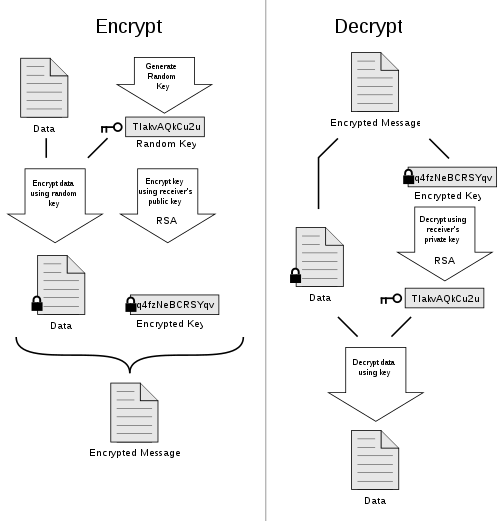
\includegraphics[width=8cm]{images/PGP_101.png}
	\caption{Schéma PGP}
	\label{fig:pgp}
\end{figure}


\section{comment citer une référence bibliographique ?}

Ceci est un exemple de citation d'un livre de Pasini~\cite{pasini2015}.

Mais aussi du site Web de Black Alps 2019~\cite{BA19} !


\section{comment faire une référence ?}

On peut aussi ajouter une référence à la section~\ref{sec:shell}.

On peut aussi ajouter une référence à l'introduction, chapitre~\ref{ch:intro}.

Comme montre la Figure~\ref{fig:pgp}, on peut référencer une figure.


\section{comment afficher une commande simple ou du bash}

Utiliser la commande \com{com}.

Exemple : Test d'une commande bash shell \com{ls} : 

Utiliser l'environnement \com{shellcmd}.

\begin{shellcmd}
$> ls -al test_underscore $$* "coucou"
\end{shellcmd}
Bli bLa


\section{Commande Shell}
\label{sec:shell}

Voici comment faire une mise en forme de commande SHELL.

Utiliser l'environnement \com{listingsbox}.
\begin{description}
 \item[1er paramètre:] le ype de shell, ici "console"
 \item[2ème paramètre:] le nom à donner à la box
\end{description}

\begin{listingsbox}{console}{Exemple de commande shell avec réponse}
root@kali:~$ bunzip2 data-decrypted.bin
bunzip2: Can't guess original name for data-decrypted.bin -- using
data-decrypted.bin.out
\end{listingsbox}


\section{Code inclus en direct dans le latex}

Utiliser l'environnement \com{sourcebox}.
\begin{description}
 \item[1er paramètre:] le ype de shell, ici "c"
 \item[2ème paramètre:] le nom à donner à la box
\end{description}

\begin{sourcebox}{c}{Exemple de code C}
#include <stdio.h>

int main(int argc, char* argv[])
{
   printf("Hello World!\n");
   return 0;
}
\end{sourcebox}



\section{Code à partir d'un fichier}

Utiliser la commande \com{inputsourcecode}.
\begin{description}
 \item[1er paramètre:] le ype de shell, ici "c"
 \item[2ème paramètre:] le nom du fichier source, "\path{source_code/example.c}"\\ Egalement exemple de la commande \com{path}.
 \item[3ème paramètre:] le nom à donner à la box
\end{description}


%% Inclure du code source d'un fichier externe
%% 1er paramètre: langage du code
%% 2ème paramètre: le path du fichier source
%% 3ème paramètre: le titre de la box
\inputsourcecode{c}{"source_code/example.c"}{example.c}

Même exemple, mais en spécifiant les lignes 4 à 8 :
\inputsourcecode[firstline=4,lastline=8]{c}{"source_code/example.c"}{example.c}
